\section{Overview and experimental design}
\label{research-design-and-methodology:overview-and-experimental-design}

The design answers two questions, and this chapter is the plan the rest of the thesis carries out: it fixes what is varied, what is held constant, how each outcome is measured in principle, and how the resulting samples are analyzed. The first question asks how the cloud-native combination of GeoParquet and DuckDB compares with the traditional alternatives, PostGIS and Shapefile, in wall-clock query time, network transfer, and operational cost, evaluated across spatial intersection predicates, distance-based nearest-neighbor search, and bounding-box range filtering on Norwegian building data at small and large dataset tiers. The second asks, for a national-scale spatial join on the same data, how broadcast-join and partitioned-join execution strategies on Apache Sedona compare against single-node PostGIS and DuckDB in wall-clock time, scaling behavior, network transfer, and operational cost across the same tiers.

Three methodological commitments separate this design from the prior benchmarks reviewed in Chapter~\ref{ch:related-work}. First, end-to-end network transfer is treated as a primary outcome and measured directly at the client, instead of being inferred from format internals or omitted. Second, cloud-native and traditional configurations are compared on an identical workload using identical data, so that any observed difference traces to the format-and-engine pairing and not to a difference in inputs. Third, single-node and distributed engines sit within one comparison framework, reported on the same axes of time, transferred bytes, and cost. Reporting both on shared axes lets the question of when distribution repays its coordination overhead be answered against a single-node reference rather than asserted. Section~\ref{background:cloud-native-data-architecture:distributed-and-non-distributed-computation} establishes that a distributed engine outperforms a single-node one only once the dataset or computation is large enough to justify its coordination cost, and the third commitment turns that premise into a measurable comparison.

These commitments resolve into four design cells formed by crossing two axes: cloud-native versus traditional and single-node versus distributed. The cloud-native single-node cell pairs DuckDB with GeoParquet; the traditional single-node cell uses PostGIS and reads Shapefiles locally; the cloud-native distributed cell uses Sedona over GeoParquet. Because the comparison turns on the format-and-engine pairing, the cells are stated at that level and laid out in Figure~\ref{fig:design-space}. Their concrete realization, including the compute platform, storage layout, and engine versions, is an implementation detail described in Chapter~\ref{ch:system-architecture-and-implementation}.

\begin{figure}[H]
    \centering
    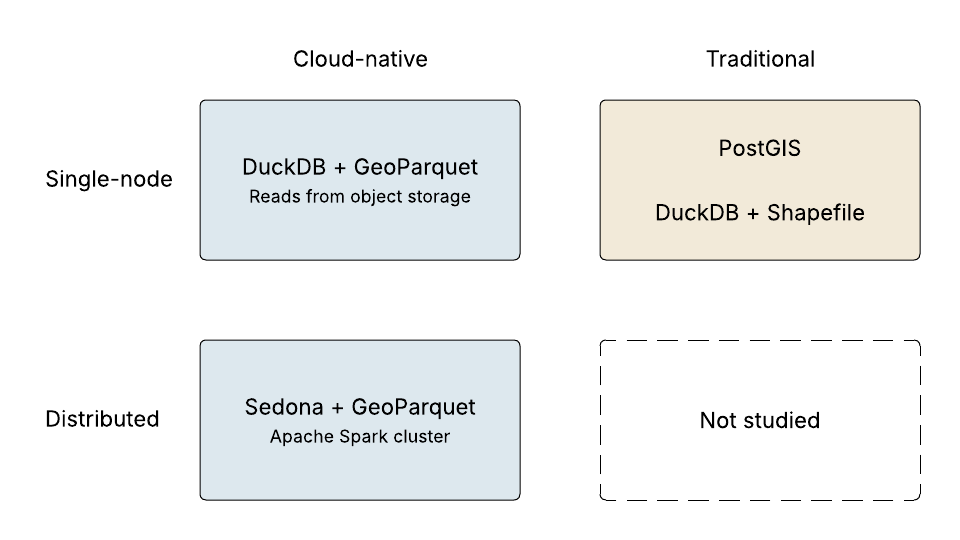
\includegraphics[width=0.85\textwidth]{Chapters/04-research-design-and-methodology/sub-chapters/figures/04-design-space.png}
    \caption[The four design cells of the experimental design]{The experimental design space, formed by crossing the cloud-native/traditional axis with the single-node/distributed axis. Three cells are populated by format-and-engine configurations; the traditional distributed cell is left unstudied, as no traditional format targets a distributed run-time in this comparison.}
    \label{fig:design-space}
\end{figure}

\subsection{Factors and levels}
\label{research-design-and-methodology:overview-and-experimental-design:factors-and-levels}

The two research questions vary different factors. \acrshort{rq}1 varies a single factor, the configuration, across four levels: DuckDB over GeoParquet, PostGIS, DuckDB over Shapefile, and Sedona over GeoParquet. \acrshort{rq}2 varies the worker count of the distributed engine across five levels, from 2 to 16 nodes, tracing how the spatial join scales with increasing parallelism. Both questions treat the workload as a secondary factor, with the query patterns and their definitions given in Section~\ref{research-design-and-methodology:workloads}. The dataset, the regions it covers, the client compute sizing, the client process that issues each query, and the access protocol are held constant across every level. A difference in an outcome then reflects the factor under test rather than a difference in inputs or in the measurement apparatus. Table~\ref{tab:methodology:factors} summarizes the factors, their levels, and the question each addresses.

\begin{table}[H]
    \centering
    \begin{tabular}{@{}l l p{6.5cm} l@{}}
        \toprule
        \textbf{Factor} & \textbf{Role} & \textbf{Levels} & \textbf{RQ} \\
        \midrule
        Configuration & Varied      & DuckDB + GeoParquet, PostGIS, DuckDB + Shapefile, Sedona + GeoParquet & \acrshort{rq}1 \\
        Worker count  & Varied      & 2, 4, 8, 12, 16 & \acrshort{rq}2 \\
        Workload      & Varied      & See Section~\ref{research-design-and-methodology:workloads} & \acrshort{rq}1, \acrshort{rq}2 \\
        \midrule
        Dataset, regions & Constant & Identical inputs across every level & --- \\
        Client compute   & Constant & Same instance sizing and process & --- \\
        Access protocol  & Constant & Same protocol across configurations & --- \\
        \bottomrule
    \end{tabular}
    \caption[Experimental factors and controls]{Factors varied in the experiment, the controls held constant across all levels, and the research question each factor addresses.}
    \label{tab:methodology:factors}
\end{table}

\subsection{Replication and randomization}
\label{research-design-and-methodology:overview-and-experimental-design:replication-and-randomization}

Each query runs as $N$ warmup iterations followed by $M$ timed iterations, with the warmup results discarded. Warmup primes caches and connection state, so the timed iterations measure an engine in steady operation rather than its cold start. The count $M$ is calibrated per workload: cheap high-frequency queries receive many iterations, the expensive national-scale join only a few. Every workload then yields a sample large enough to characterize its distribution without spending run-time on iterations that add no information.

Within each benchmark run, a seeded random number generator randomizes the execution order of the experiments, and the seed is reused across runs for reproducibility. Randomizing the order of test and control measurements on the same instance reliably detects small slowdowns under cloud variability \parencite{laaber2019_software_microbenchmarking_cloud}. The bootstrap that the iteration-count rule of Section~\ref{research-design-and-methodology:workloads:iteration-counts} applies after each timed iteration draws on a separate generator, seeded deterministically from the run and query identifiers through a hash, so the point at which a run stops is reproducible whenever those identifiers recur. Configurations compared on the same workload are also paired and launched concurrently on identically provisioned client instances. The two members of a comparison then share the same short-term conditions, reducing the time-of-day variance between them rather than leaving it to vary across runs \parencite{laaber2019_software_microbenchmarking_cloud}. The distributed configuration is the one exception to the warmup discipline. Because each of its runs provisions a fresh cluster, warmup iterations would multiply the provisioning cost without priming a persistent engine. They are therefore omitted, and the resulting variance is treated separately in Section~\ref{research-design-and-methodology:statistical-analysis}. The orchestration, container sizing, and cluster lifecycle that realize this protocol are deferred to Chapter~\ref{ch:system-architecture-and-implementation}.